\subsection{Computer interface}
An interface between the embedded controller and a computer is implemented to monitor the system, start the inverter and change the gains for the controllers. The interface is made in a simple low-level way with a predefined message structure and limited error handling. The structure can be seen in table \ref{tab:message_structure}. 


\begin{table}[H]
\centering
\begin{tabular}{|l|c|c|c|c|c|c|}
\hline
\# character       & 1       & 2                 & 3            & 4            & 5       & 6   \\ \hline
Function      & ID  & Read / Write                     & \multicolumn{4}{c|}{Value}               \\ \hline
Valid Values & $0\rightarrow 9$ & 'r'/'w'  & \multicolumn{4}{c|}{$0\rightarrow 9999$} \\ \hline
\end{tabular}
\caption{Structure of the interface messages from the computer to the embedded controller.}
\label{tab:message_structure}
\end{table}

The first character of the message contains an ID of the variable that the message is referring to. The IDs of all variables included can be seen in table \ref{tab:variable_ids}.

The second character describes if the message is a read or write command.

The third till sixth character are only used for the write command. They contain the value to which the variable should be changed to. The format of the value can be seen in table \ref{tab:variable_ids}. To handle digits especially for the controller gains the values from $0000 \rightarrow 9999$ are mapped to $00.00 \rightarrow 99.99$ before being added to the controller.


\begin{table}[H]
\centering
\begin{tabular}{|l|llll|} \hline
ID & Valid values                                               & Valid commands & Variable    & Unit       \\   \hline
0  & \begin{tabular}[c]{@{}l@{}}0 = Stop\\1 = Run \end{tabular} & 'r'/'w'        & Inverter state & - \\ \hline
1  & -                                                          & 'r'            & Speed       & Hz \\ \hline
2  & $0 \rightarrow 9999$                                                     & 'r'/'w'        & Ki\_D       & \begin{tabular}[c]{@{}l@{}}$1/100$ \\ \textit{Example: 1234 = 12.34}\end{tabular} \\ \hline
3  & $0 \rightarrow 9999$                                                     & 'r'/'w'        & Kp\_D       & \begin{tabular}[c]{@{}l@{}}$1/100$ \\ \textit{Example: 1234 = 12.34}\end{tabular} \\ \hline
4  & $0 \rightarrow 9999$                                                     & 'r'/'w'        & Ki\_Q       & \begin{tabular}[c]{@{}l@{}}$1/100$\\ \textit{Example: 1234 = 12.34}\end{tabular}  \\ \hline
5  & $0 \rightarrow 9999$                                                     & 'r'/'w'        & Kp\_Q       & \begin{tabular}[c]{@{}l@{}}$1/100$\\ \textit{Example: 1234 = 12.34}\end{tabular}  \\ \hline
\end{tabular}
\caption{List of variables that can be accessed through the communication between a computer and the embedded controller.}
\label{tab:variable_ids}
\end{table}

An example of how the communication can be seen on figure \ref{fig:pc_interface}. 

Line 1 is a command to write the value $03.46$ to the variable with ID=2 which is \textit{Ki\textunderscore D}. 

Line 2 is a read command of the same variable. 

Line 3 is the reply from the embedded system.

Line 5 is a write command to write the value \textit{1} to the variable with ID=0 which translates to sending a start command to the inverter. Line 6 and 7 are the same as 2 and 3 but for the inverter state.

Line 9 is a command to write the value $15.23$ to the gain \textit{Ki\textunderscore Q}.

\begin{figure}[H]
	\centering
	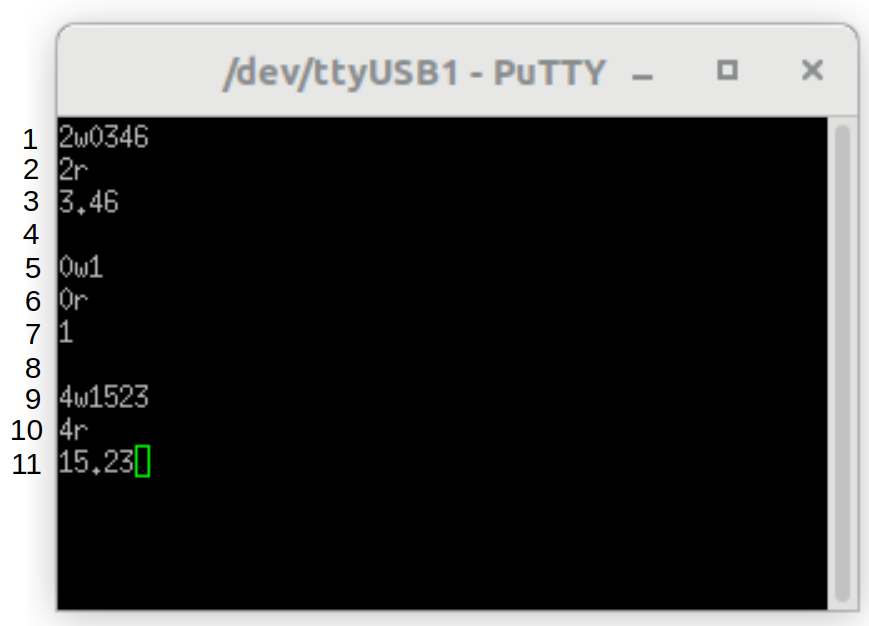
\includegraphics[width=0.65\linewidth]{pictures/software/pc_interface_terminal.png}
	\caption{Example of the computer interface used for communication between the embedded controller and a computer.}
	\label{fig:pc_interface}
\end{figure}